\begin{frame}
    \frametitle{Audioverarbeitung}
    \framesubtitle{Spektrogramm}
    Visualisierung von Signalen in einem Spektrogramm:
    \begin{itemize}
        \item Visualisiert den zeitlichen Verlauf des Frequenzspektrums
        \item Für jeden Zeitpunkt eine Fourier Analyse
        \item Signalanalyse, Musikerkennung
    \end{itemize} 
    \begin{columns}
        \begin{column}{120px}
            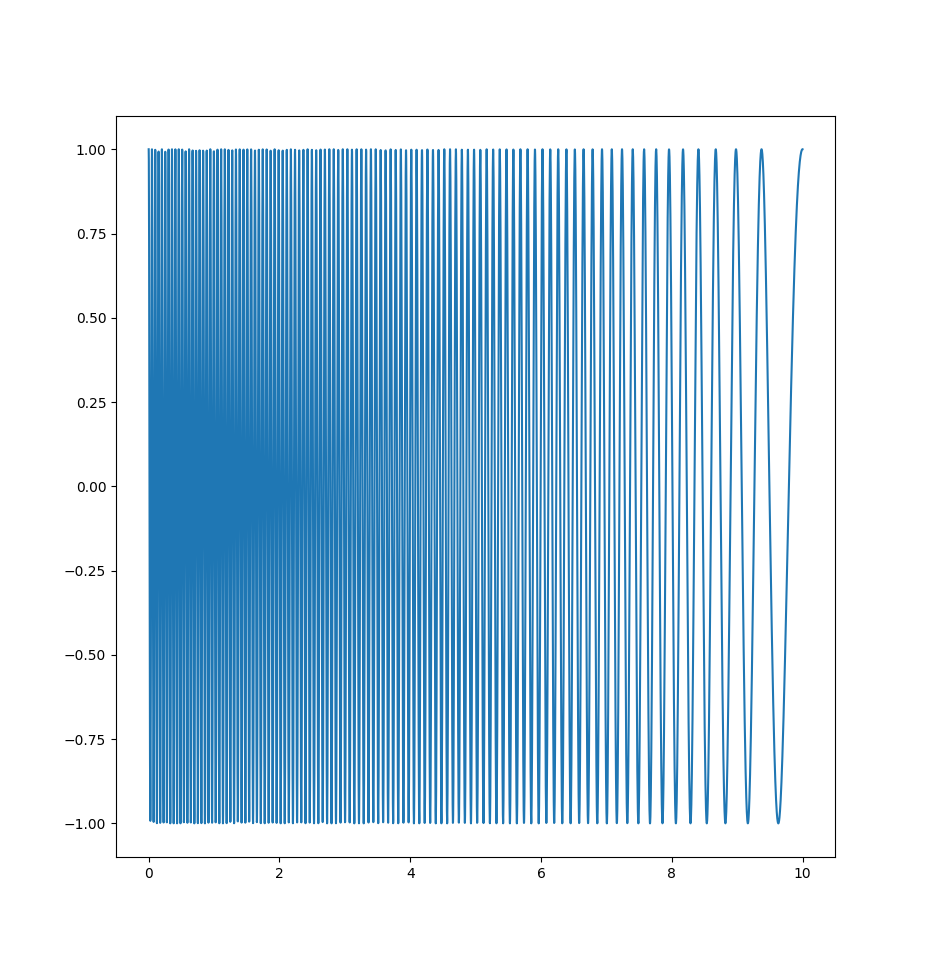
\includegraphics[width=120px]{images/04-applications-audio-chirp.png}
        \end{column}
        \hspace*{-25px}
        \begin{column}{5px}
            $\rightarrow$
        \end{column}
        \hspace*{-25px}
        \begin{column}{120px}
            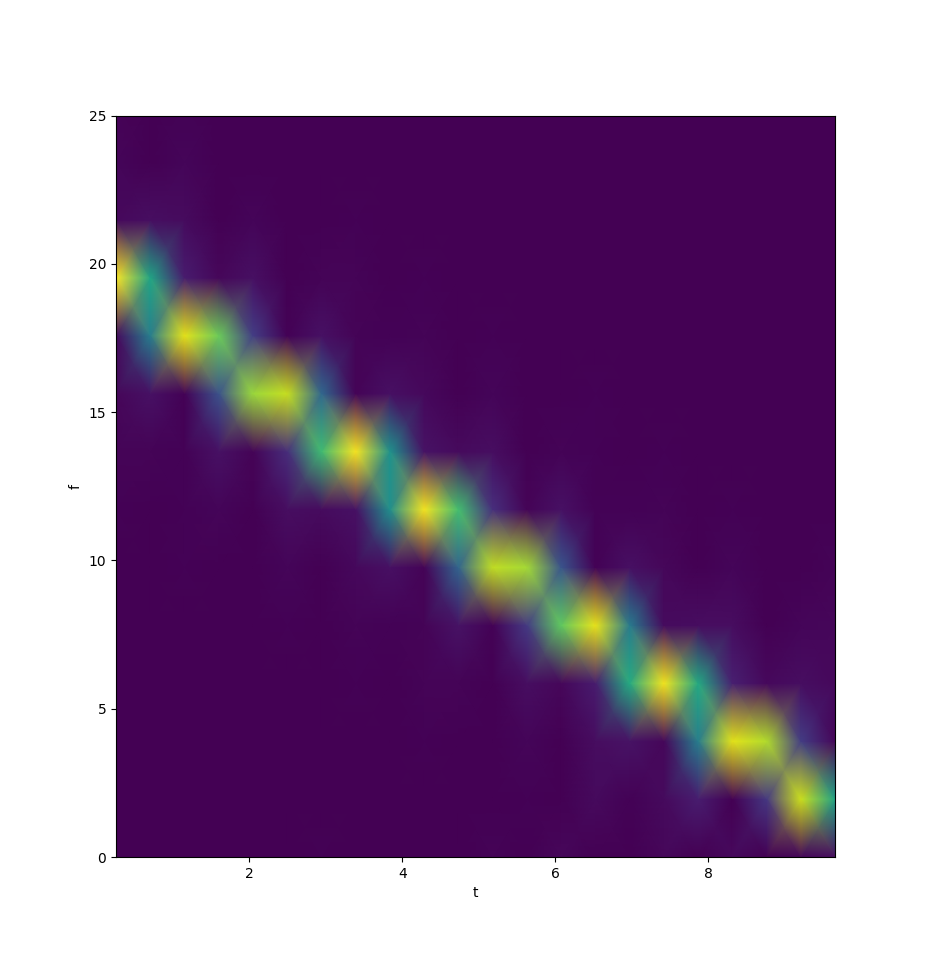
\includegraphics[width=120px]{images/04-applications-audio-chirp-spectrogram.png} 
        \end{column}
    \end{columns}
\end{frame}

\begin{frame}
    \frametitle{Audioverarbeitung}
    \framesubtitle{Frequenzfilterung}
    Filtern von Frequenzen:
    \begin{itemize}
        \item Identifizieren von Störfrequenzen
        \item Eliminierung von diesem aus Frequenzspektrum
        \item Inverse Fourier Transformation anwenden
    \end{itemize}
\end{frame}

\begin{frame}
    \frametitle{Anwendungen}
    \framesubtitle{Audio}

    \begin{columns}
        \begin{column}{160px}
            \centering
            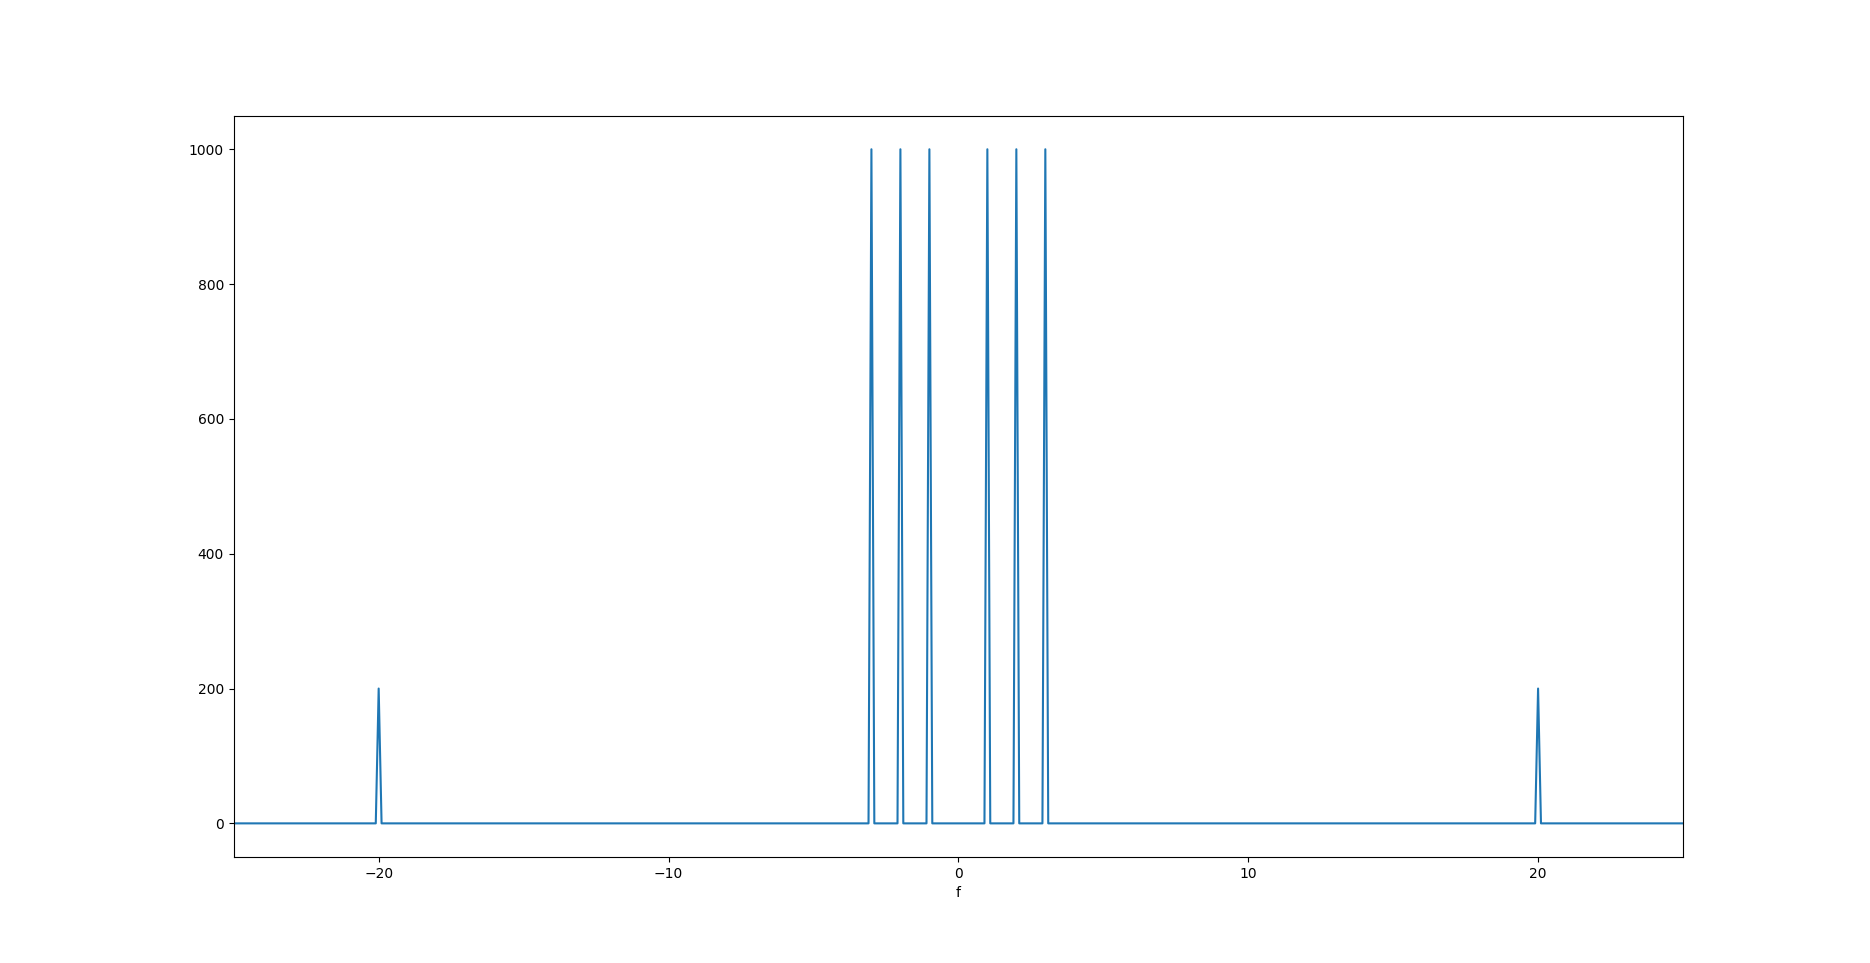
\includegraphics[width=160px]{images/04-applications-audio-noisy-signal-ft.png}
            $\downarrow$
            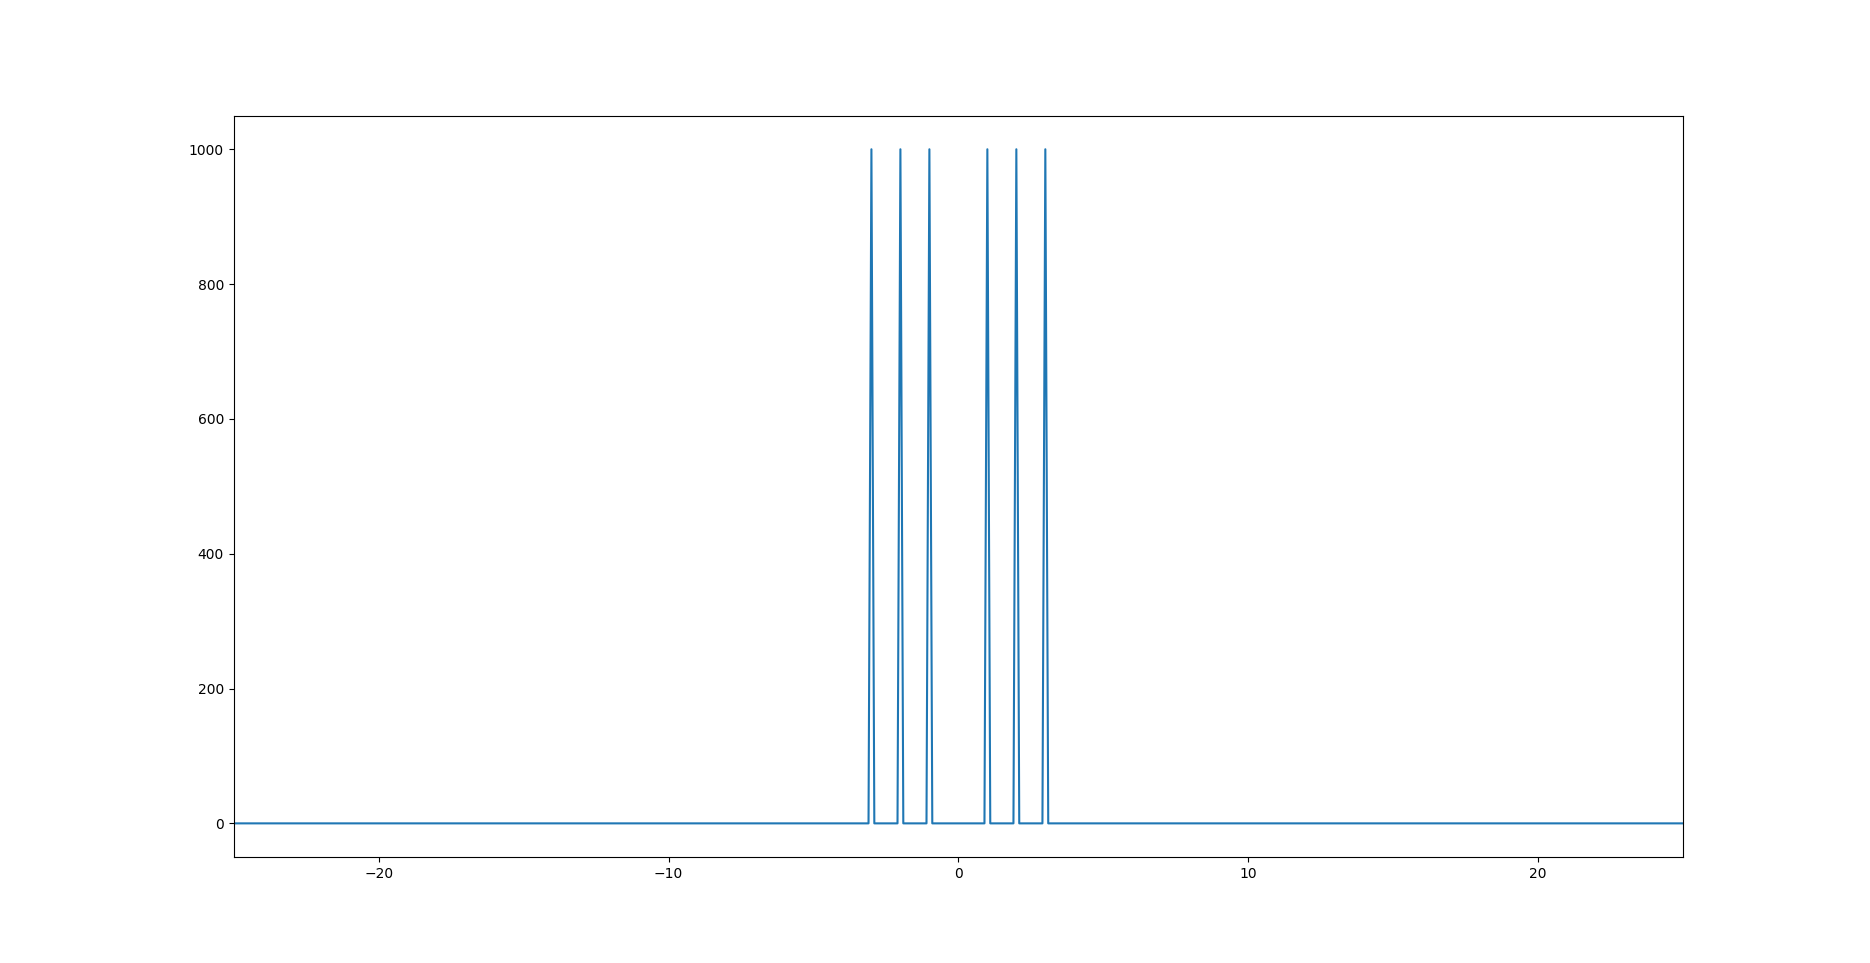
\includegraphics[width=160px]{images/04-applications-audio-clean-signal-ft.png}
        \end{column}
        \hspace*{-25px}
        \begin{column}{1px}
            \vspace*{-13px}
            \begin{align*}
                \overset{FT}\longleftarrow \\ \\ \\ \\ \\ \\
                \overset{IFT}\longrightarrow
            \end{align*}
        \end{column}
        \hspace*{-25px}
        \begin{column}{100px}
            \centering
            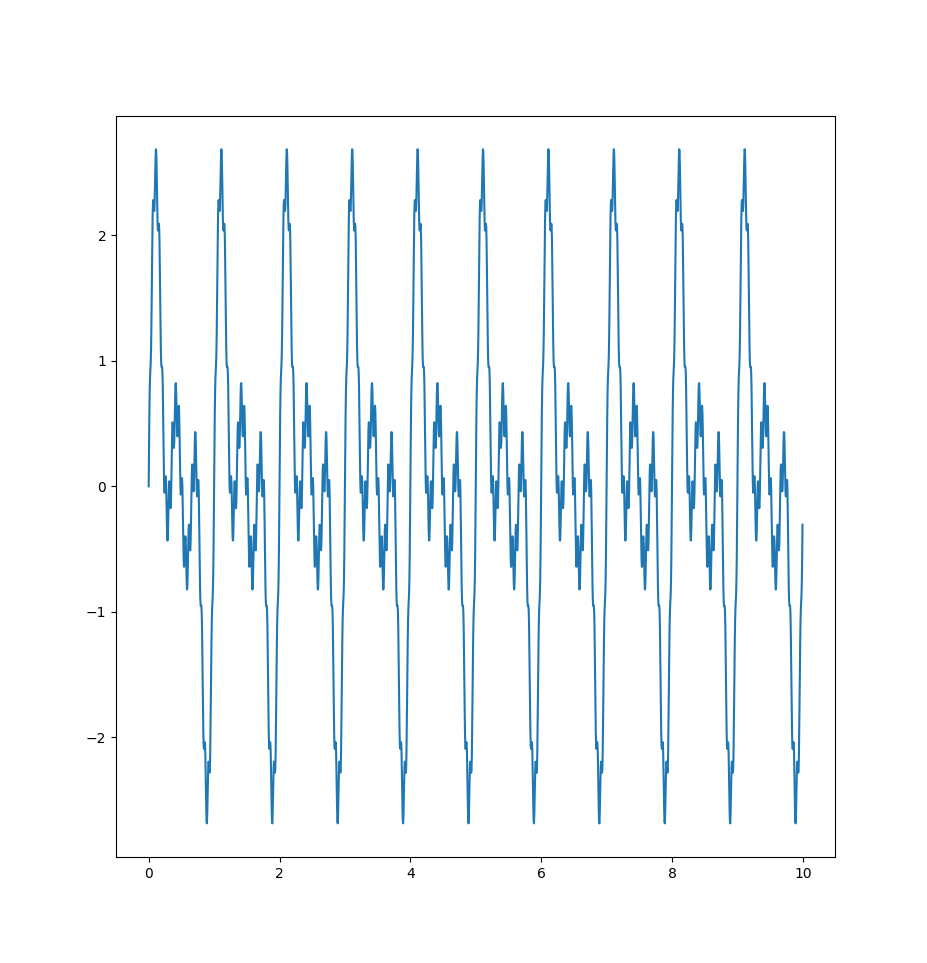
\includegraphics[width=100px]{images/04-applications-audio-noisy-signal.png}
            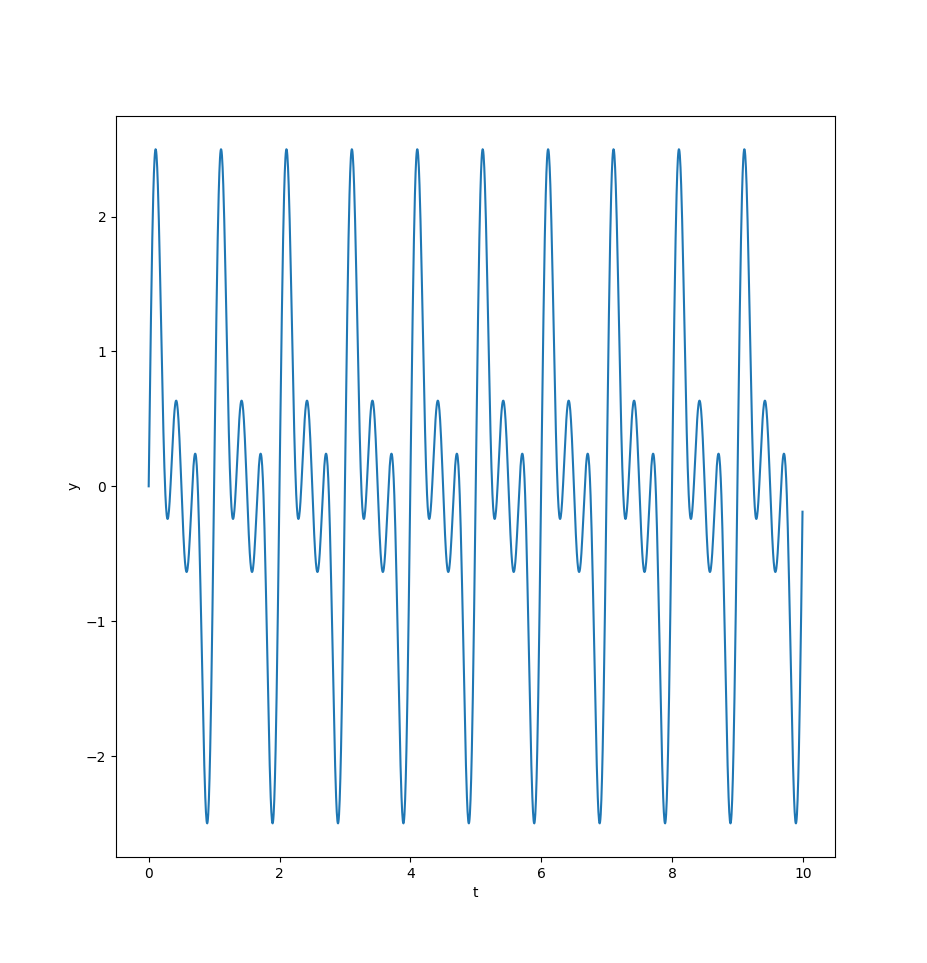
\includegraphics[width=100px]{images/04-applications-audio-clean-signal-ift.png}
        \end{column}
    \end{columns}
\end{frame}

\begin{frame}
    \frametitle{Bildverarbeitung}
    \framesubtitle{Voraussetzungen}

    \begin{itemize}
        \item Benötigt eine 2-Dimensionale Fourier Transformation
    \end{itemize}
    \begin{align*}
        (\mathcal{F} b)(k, l)=\int_{-\infty}^{\infty}{\int_{-\infty}^{\infty}{b(x, y)\cdot e^{-i2\pi (kx+ly)} \ dx}\ dy}
    \end{align*}
    Oder diskret:
    \begin{align*}
        (\mathcal{F} b)(k, l)=\sum_{x=0}^{X-1}{\sum_{y=0}^{Y-1}{b(x,y)\cdot e^{-i(\omega_kx+\omega_ly)}}}
    \end{align*}
\end{frame}

\begin{frame}
    \frametitle{Bildverarbeitung}
    \framesubtitle{Eigenschaften der 2D-FT}

    \begin{itemize}
        \item Der Fourier Raum hat die gleiche Dimension wie das Bild
        \item x-Achse und y-Achse beschreiben Frequenzen
        \item Die Farbe eines Pixels beschreibt die Magnitude/Phase
        \item Punktsymmetrisch um den Ursprung
    \end{itemize}
\end{frame}

\begin{frame}
    \frametitle{Bildverarbeitung}
    \framesubtitle{2D Fourier Raum}
    \centering
    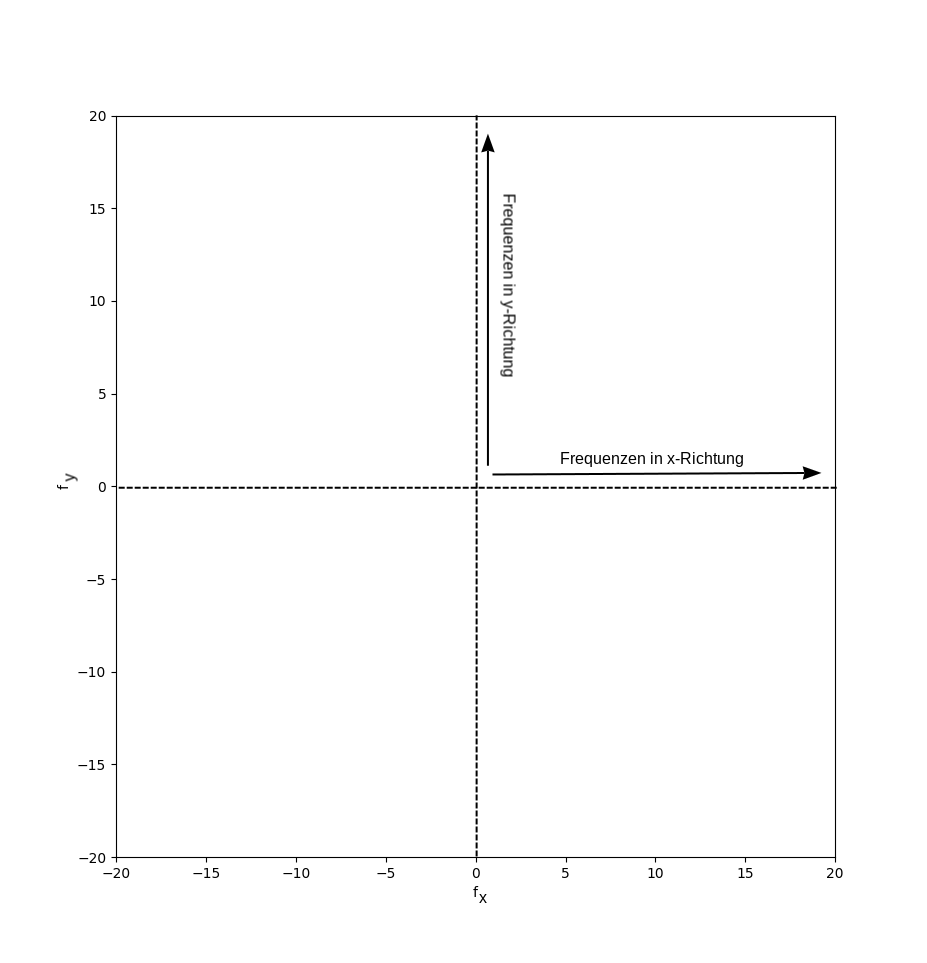
\includegraphics[width=170px]{images/04-applications-fourier-space-empty.png}
\end{frame}

\begin{frame}
    \frametitle{Bildverarbeitung}
    \framesubtitle{2D Fourier Raum}
    \centering
    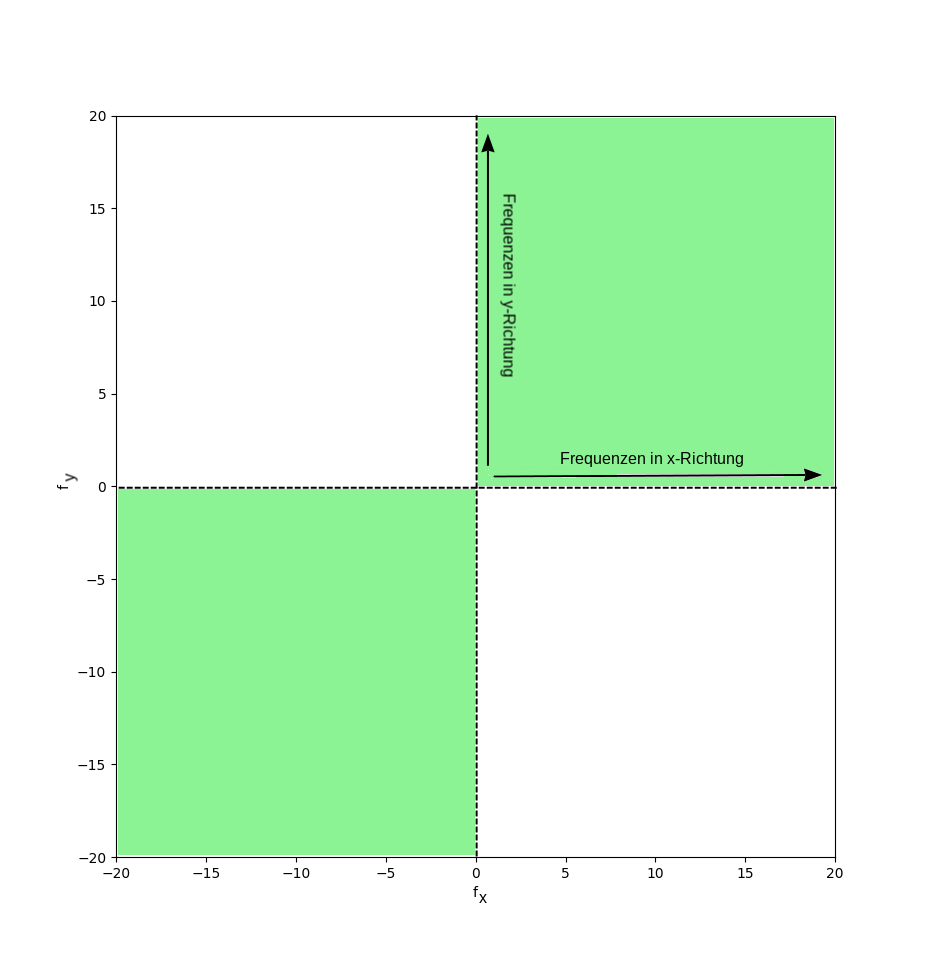
\includegraphics[width=170px]{images/04-applications-fourier-space-empty-1.png}
\end{frame}

\begin{frame}
    \frametitle{Bildverarbeitung}
    \framesubtitle{2D Fourier Raum}
    \centering
    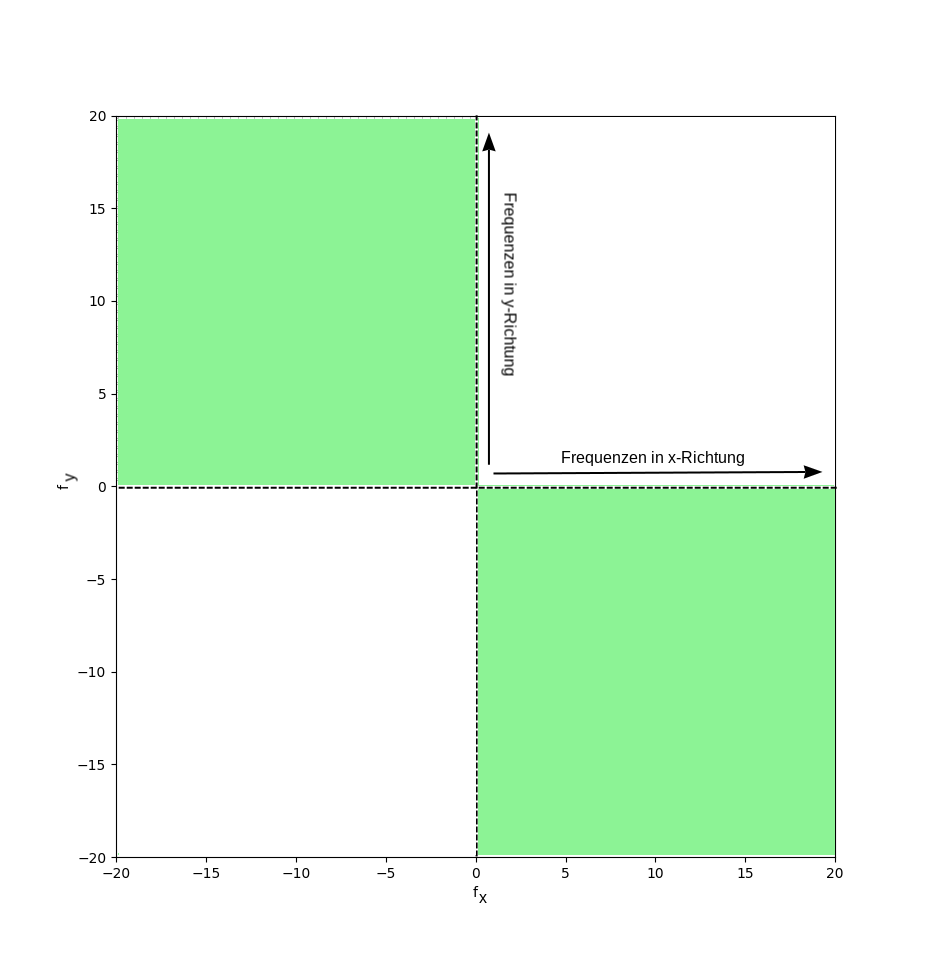
\includegraphics[width=170px]{images/04-applications-fourier-space-empty-2.png}
\end{frame}

\begin{frame}
    \frametitle{Bildverarbeitung}
    \framesubtitle{Fourier Transformation von einfachen Kosinusbildern}
    \begin{columns}
        \begin{column}{100px}
            \centering
            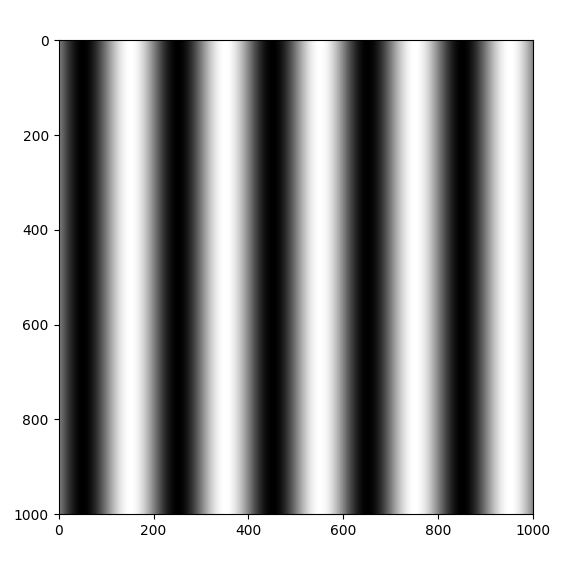
\includegraphics[width=100px]{images/04-applications-image-cos.png}
            $\downarrow$
            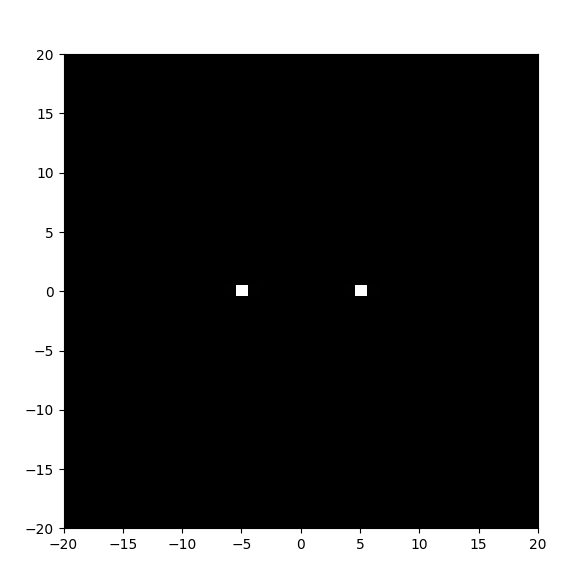
\includegraphics[width=100px]{images/04-applications-image-cos-ft.png}
        \end{column}
    \end{columns}
\end{frame}

\begin{frame}
    \frametitle{Bildverarbeitung}
    \framesubtitle{Fourier Transformation von einfachen Kosinusbildern}
    \begin{columns}
        \begin{column}{100px}
            \centering
            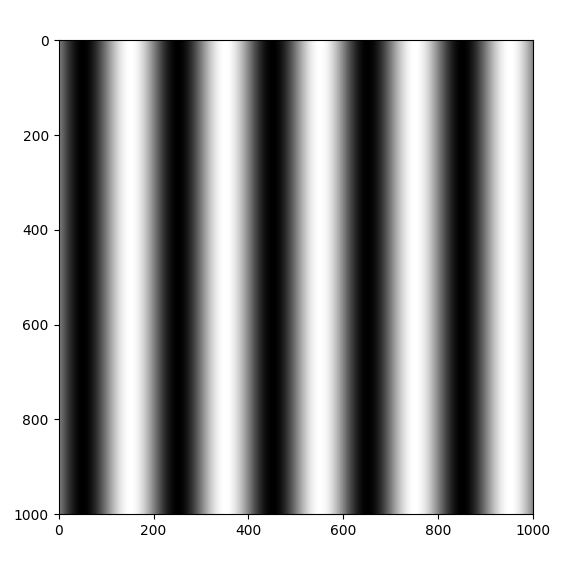
\includegraphics[width=100px]{images/04-applications-image-cos.png}
            $\downarrow$
            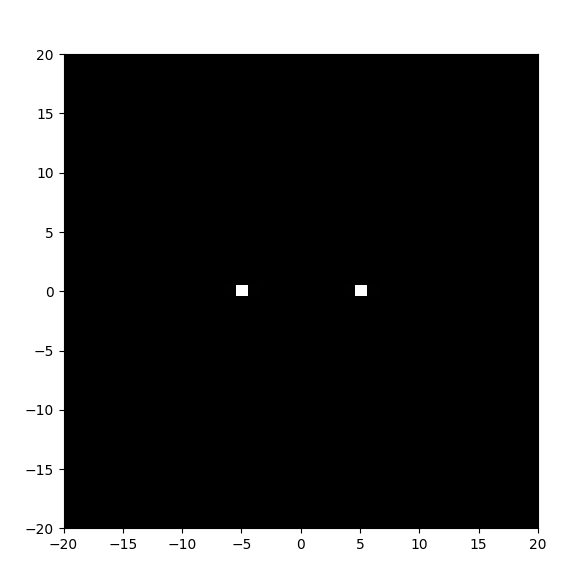
\includegraphics[width=100px]{images/04-applications-image-cos-ft.png}
        \end{column}
        \begin{column}{100px}
            \centering
            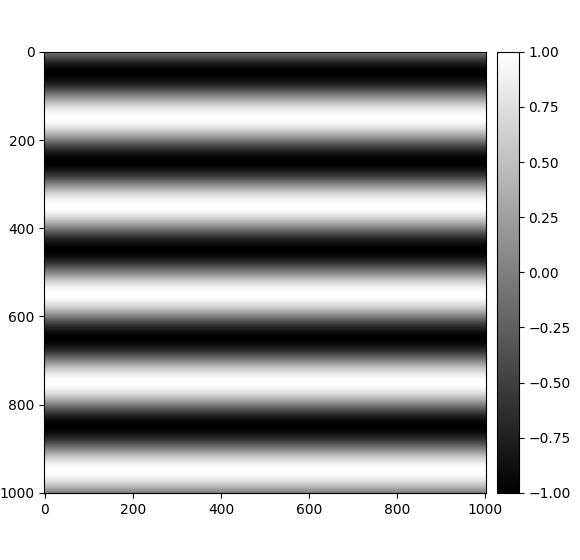
\includegraphics[width=100px]{images/04-applications-image-cos-rot.png}
            $\downarrow$
            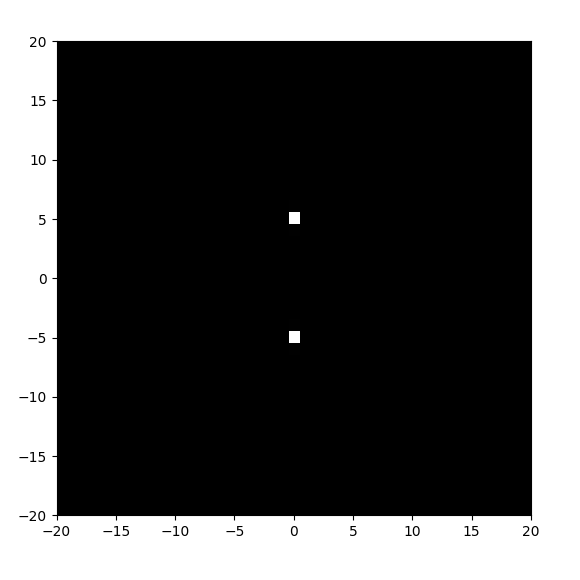
\includegraphics[width=100px]{images/04-applications-image-cos-rot-ft.png}
        \end{column}
    \end{columns}
\end{frame}

\begin{frame}
    \frametitle{Bildverarbeitung}
    \framesubtitle{Fourier Transformation von einfachen Kosinusbildern}
    \begin{columns}[t]
        \begin{column}{100px}
            \centering
            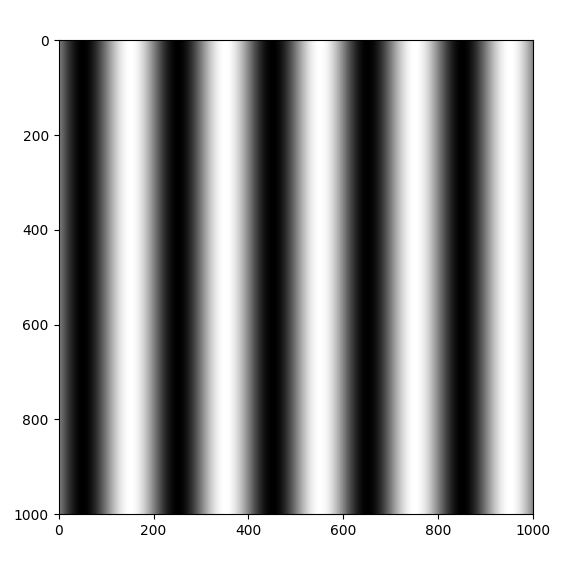
\includegraphics[width=100px]{images/04-applications-image-cos.png}
            $\downarrow$
            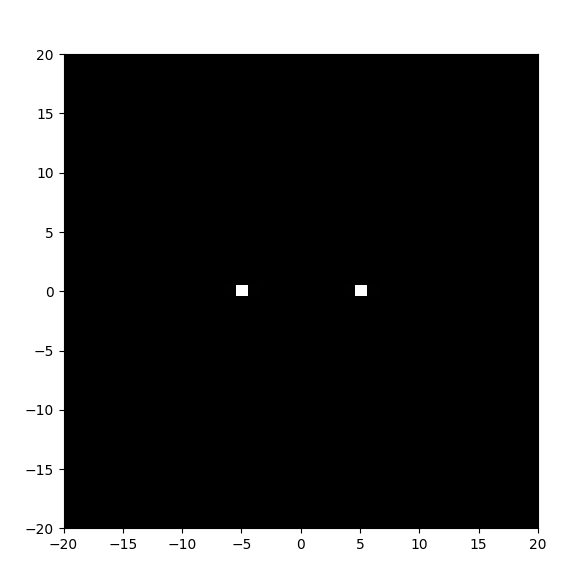
\includegraphics[width=100px]{images/04-applications-image-cos-ft.png}
        \end{column}
        \begin{column}{100px}
            \centering
            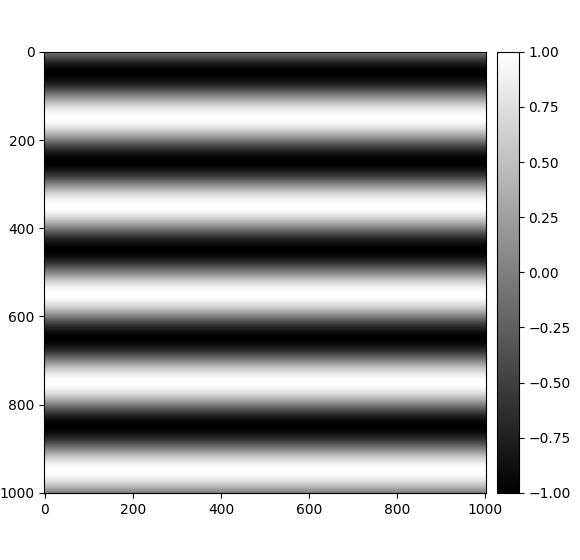
\includegraphics[width=100px]{images/04-applications-image-cos-rot.png}
            $\downarrow$
            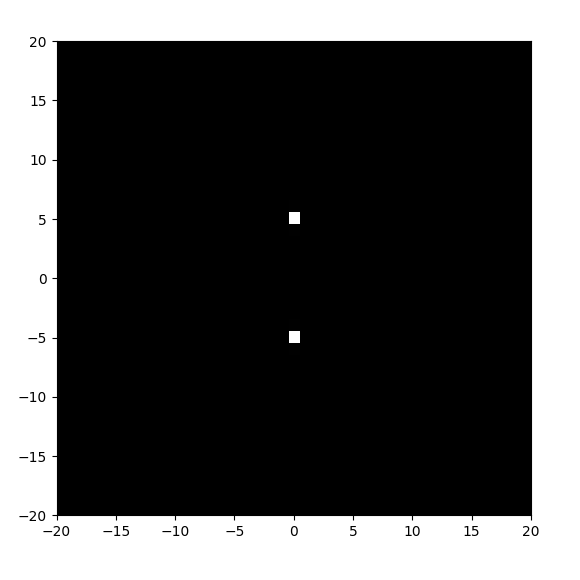
\includegraphics[width=100px]{images/04-applications-image-cos-rot-ft.png}
        \end{column}
        \begin{column}{100px}
            \centering
            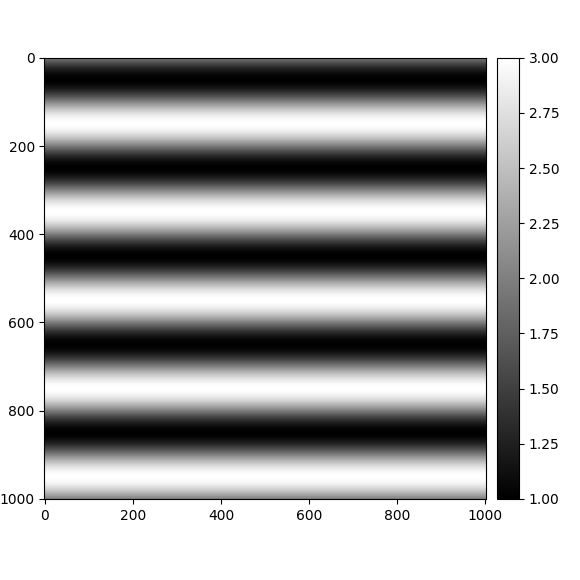
\includegraphics[width=100px]{images/04-applications-image-cos-rot-dc.png}
        \begin{tcolorbox}[halign=center, colback=white, boxrule=0pt, colframe=white, enlarge top by=-0.45cm]
            $\downarrow $ 

            \vspace{30px}
            \LARGE{?}
            \end{tcolorbox}
        \end{column}
    \end{columns}
\end{frame}

\begin{frame}
    \frametitle{Bildverarbeitung}
    \framesubtitle{Fourier Transformation von einfachen Kosinusbildern}
    \begin{columns}
        \begin{column}{100px}
            \centering
            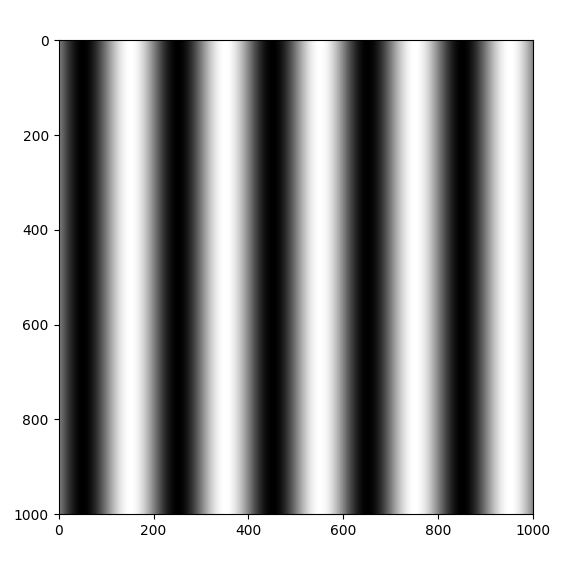
\includegraphics[width=100px]{images/04-applications-image-cos.png}
            $\downarrow$
            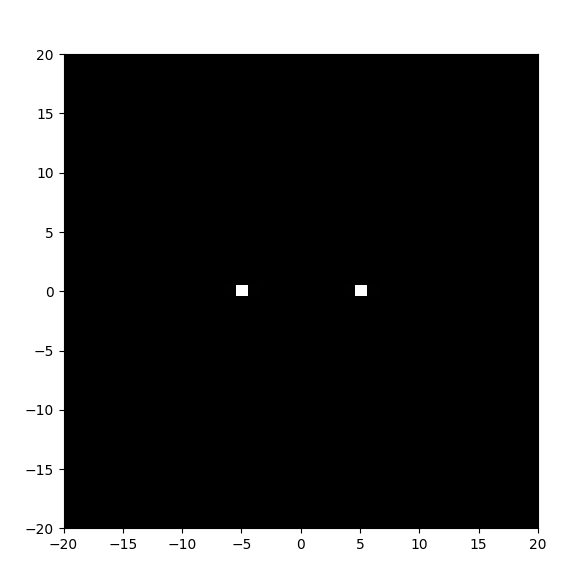
\includegraphics[width=100px]{images/04-applications-image-cos-ft.png}
        \end{column}
        \begin{column}{100px}
            \centering
            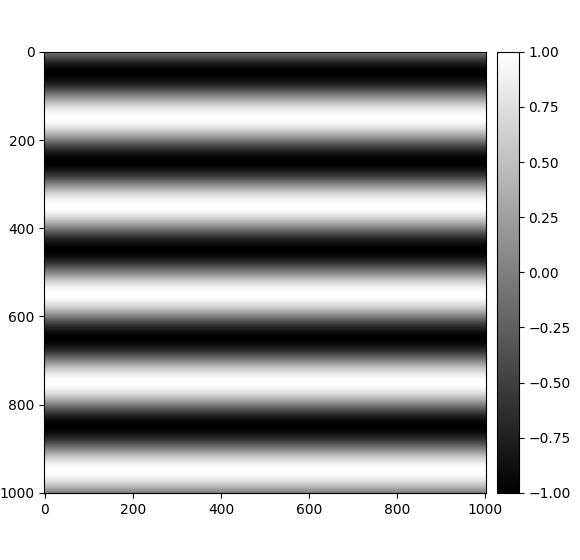
\includegraphics[width=100px]{images/04-applications-image-cos-rot.png}
            $\downarrow$
            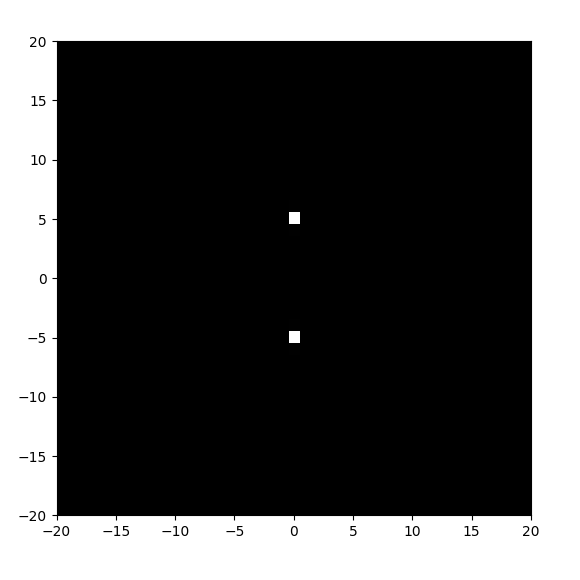
\includegraphics[width=100px]{images/04-applications-image-cos-rot-ft.png}
        \end{column}
        \begin{column}{100px}
            \centering
            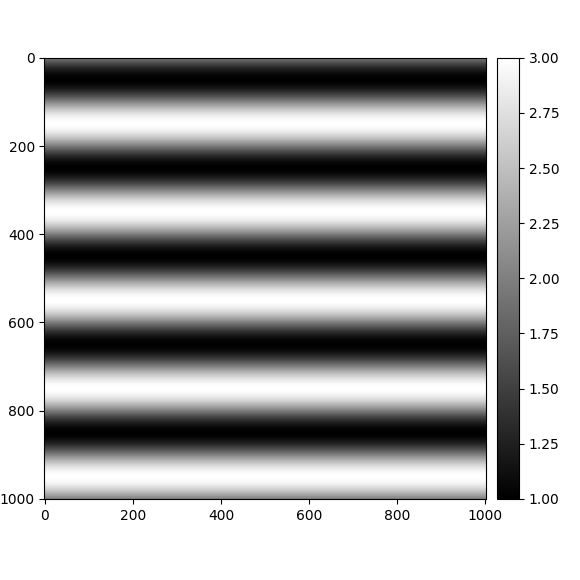
\includegraphics[width=100px]{images/04-applications-image-cos-rot-dc.png}
            $\downarrow$
            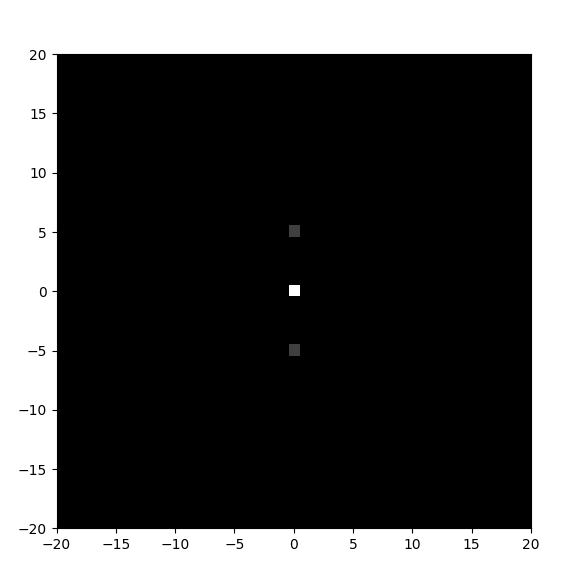
\includegraphics[width=100px]{images/04-applications-image-cos-rot-dc-ft.png}
        \end{column}
    \end{columns}
\end{frame}

\begin{frame}
    \frametitle{Bildverarbeitung}
    \framesubtitle{Schräge Kosinusbilder}
    Schräger Kosinus:
    \begin{itemize}
        \item Kanteneffekte wenn nicht periodisch
    \end{itemize}
    \begin{columns}
        \begin{column}{100px}   
            
\includegraphics[width=100px]{images/04-applications-image-cos-rot-45-0.png}
        \end{column} 
        \hspace*{-30px}
        \begin{column}{5px}
            $\rightarrow$
        \end{column}
        \hspace*{-30px}
        \begin{column}{120px}
            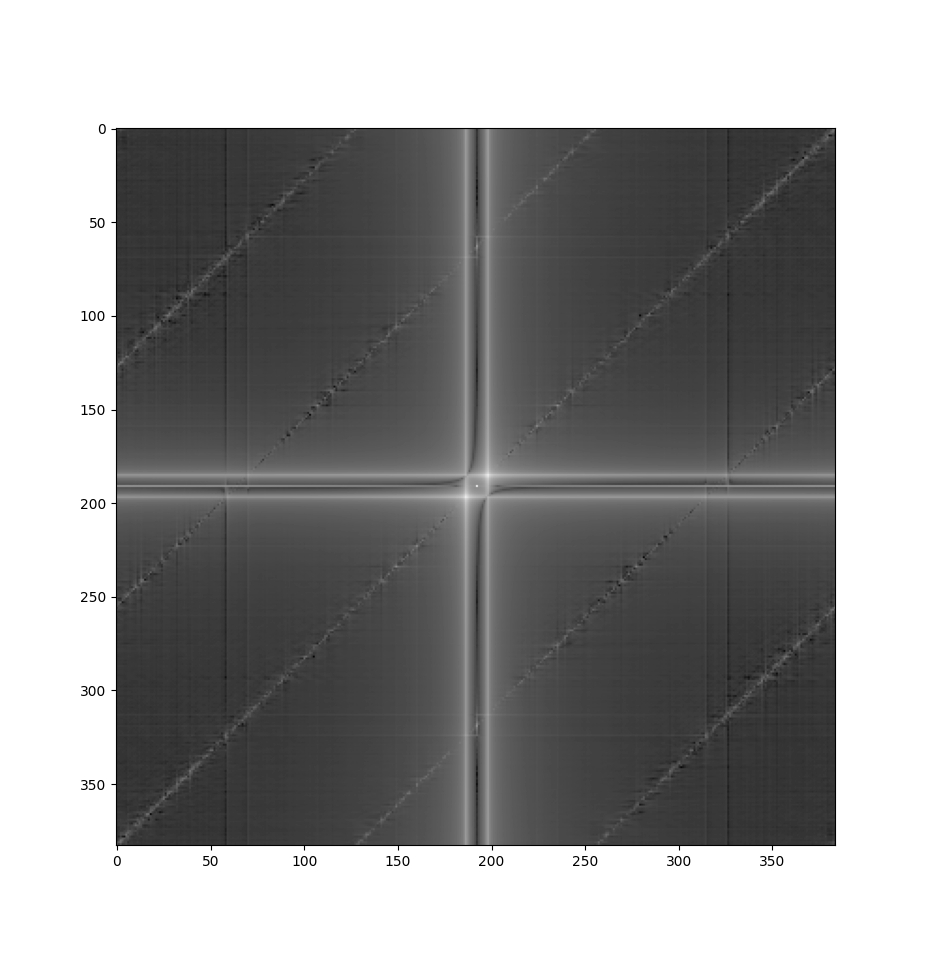
\includegraphics[width=120px]{images/04-applications-image-cos-rot-45-0-ft.png}
        \end{column}
    \end{columns}
\end{frame}

\begin{frame}
    \frametitle{Bildverarbeitung}
    \framesubtitle{Schräge Kosinusbilder}

    \begin{itemize}
        \item Die Fouriertransformation nimmt das Signal als periodisch weitergeführt an
    \end{itemize}

    \vspace{10px}
    \centering
    
\includegraphics[width=100px]{images/04-applications-image-rot-45.png}

    \vspace{5px}
    \begin{itemize}
        \item Starke Kanten
        \item Hohe diagonale Frequenzen
    \end{itemize}
\end{frame}

\begin{frame}
    \frametitle{Bildverarbeitung}
    \framesubtitle{Kanten}
    \begin{itemize}
        \item Scharfe Kanten sind mit Frequenzbändern im Fourier Raum verbunden        
        \item Für jede Kante ein Frequenzband
    \end{itemize}
    \begin{columns}
        \begin{column}{100px}
            
\includegraphics[width=100px]{images/04-applications-image-cubes.jpg}
        \end{column}
        \hspace*{-50px}
        \begin{column}{5px}
            $\rightarrow$
        \end{column}
        \hspace*{-50px}
        \begin{column}{100px}
            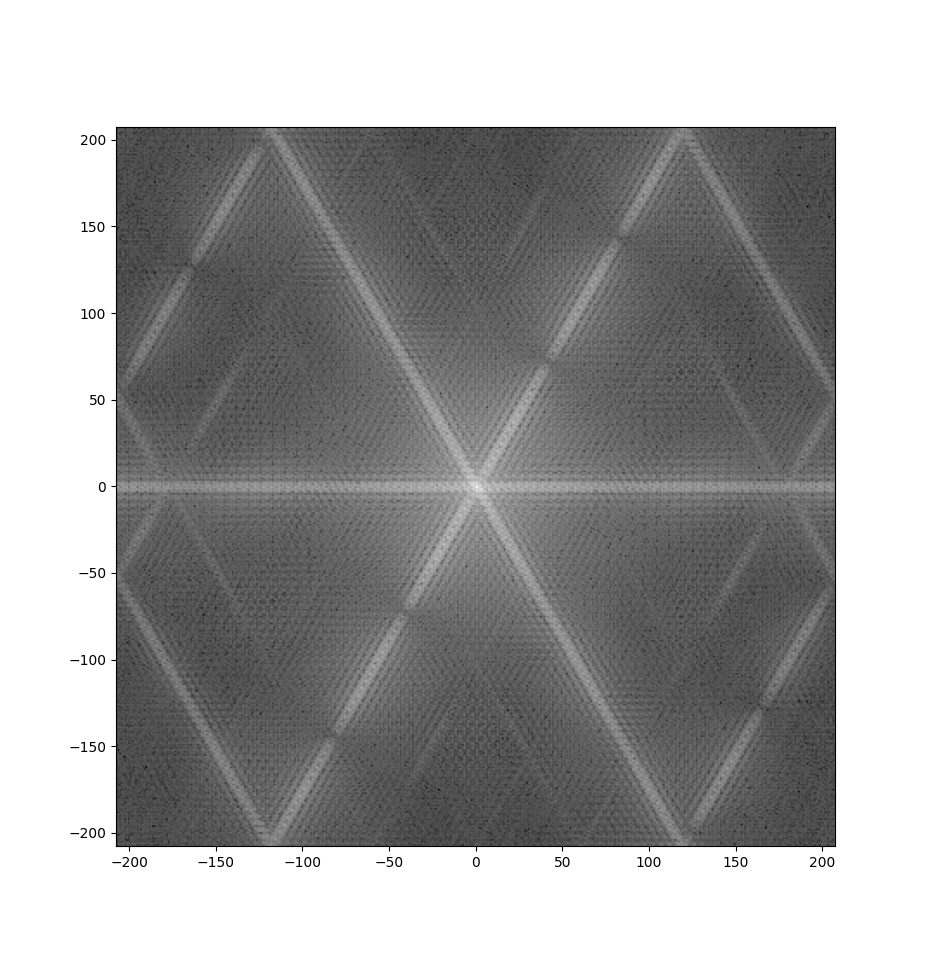
\includegraphics[width=100px]{images/04-applications-image-cubes-ft.png}
        \end{column}
    \end{columns}
\end{frame}

\begin{frame}
    \frametitle{Bildverarbeitung}
    \framesubtitle{Hochpass}
    \begin{itemize}
        \item Filtert niedrige Frequenzen aus dem Bild heraus
    \end{itemize}
    \begin{columns}[c]
        \begin{column}{90px}
            \centering
            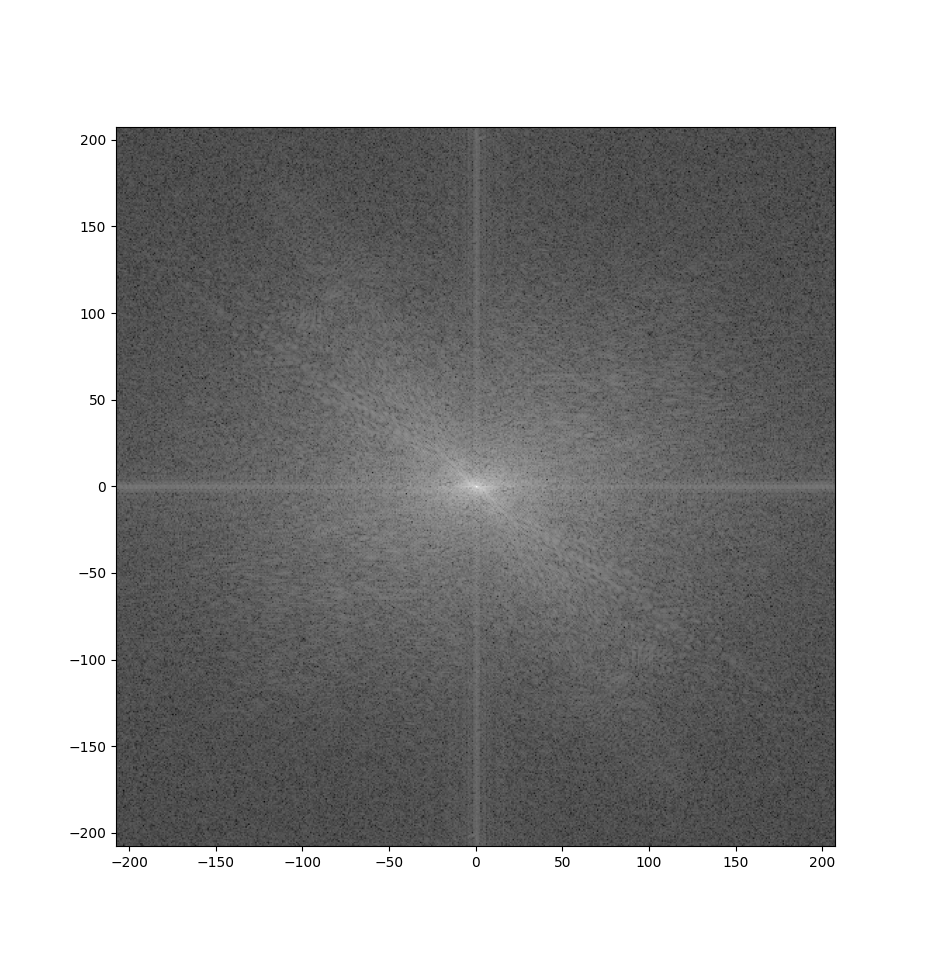
\includegraphics[width=90px]{images/04-applications-image-lena-ft.png}
            $\downarrow$
            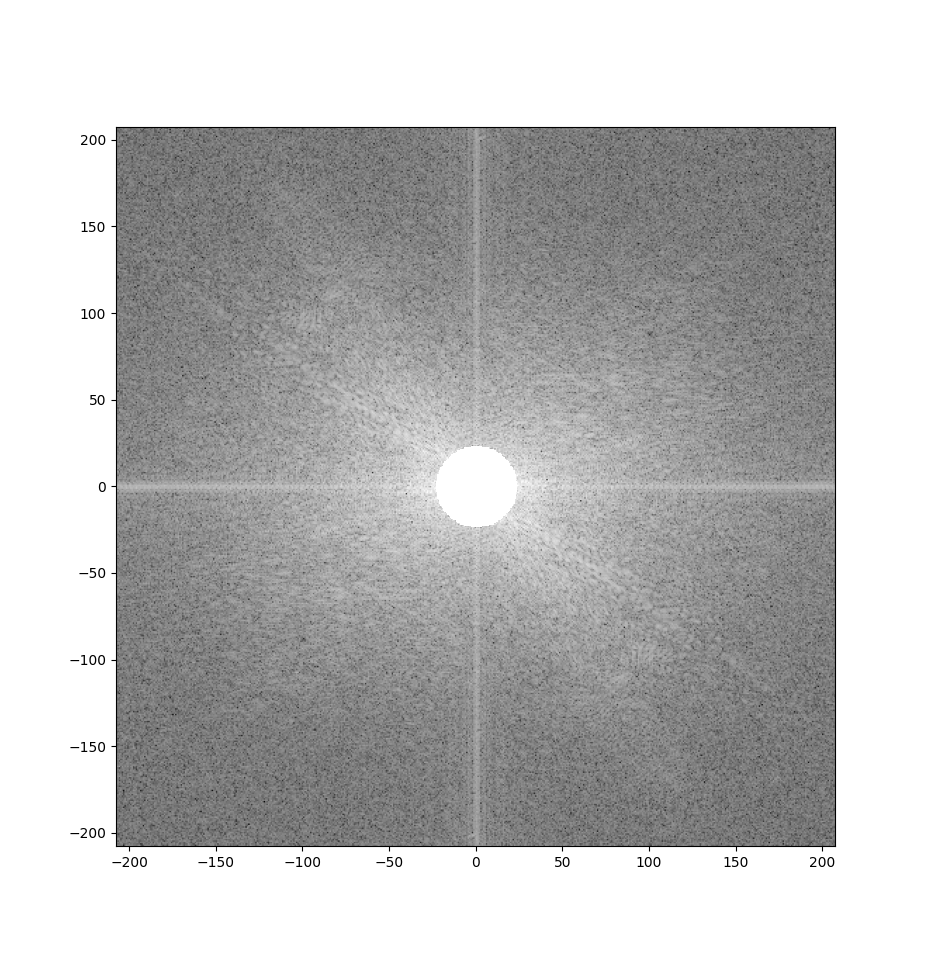
\includegraphics[width=90px]{images/04-applications-image-lena-ft-high-pass-ft.png}
        \end{column}
        \hspace*{-35px}
        \begin{column}{1px}
            \vspace*{-13px}
            \begin{align*}
                \overset{FT}\longleftarrow \\ \\ \\ \\ \\ \\
                \overset{IFT}\longrightarrow
            \end{align*}
        \end{column}
        \hspace*{-35px}
        \begin{column}{100px}
            \centering
            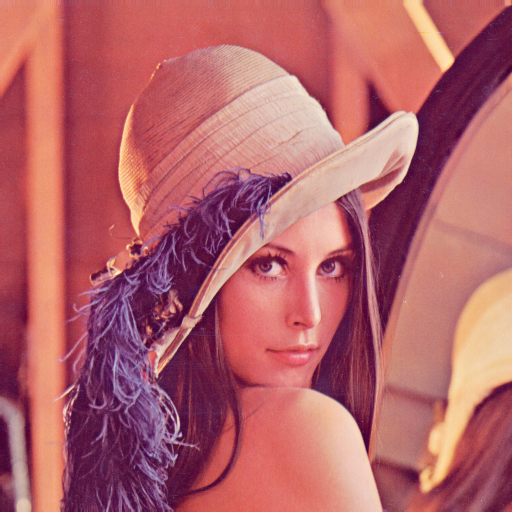
\includegraphics[width=70px]{images/04-applications-image-lena.png}
            \vspace*{-30px}
            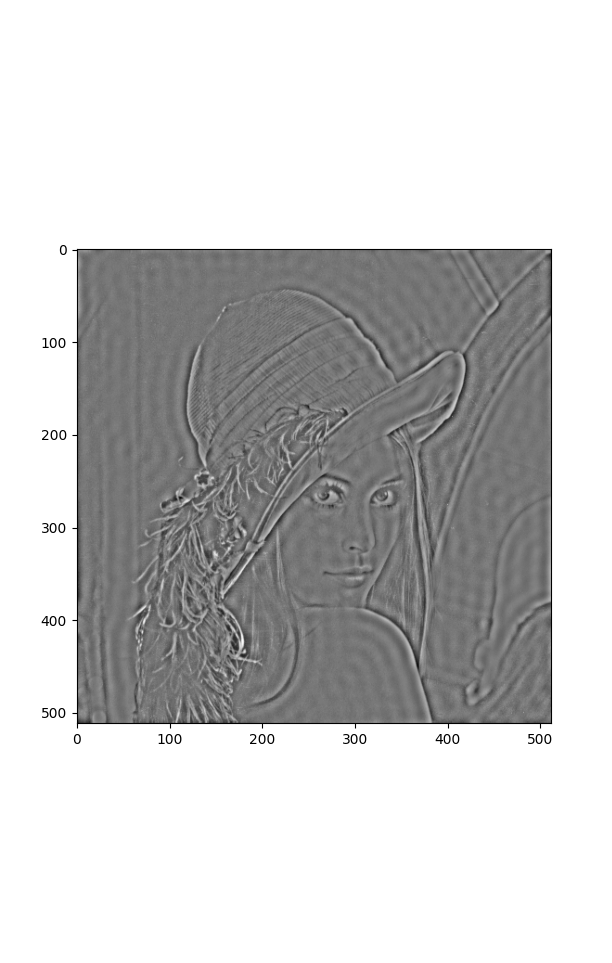
\includegraphics[width=90px]{images/04-applications-image-lena-ft-high-pass.png}
        \end{column}
    \end{columns}
\end{frame}

\begin{frame}
    \frametitle{Bildverarbeitung}
    \framesubtitle{Rauschfilterung}
    \begin{itemize}
        \item Simplifiziertes Beispiel mit nur einer Rauschfrequenz
    \end{itemize}
    \begin{columns}
        \begin{column}{120px}
            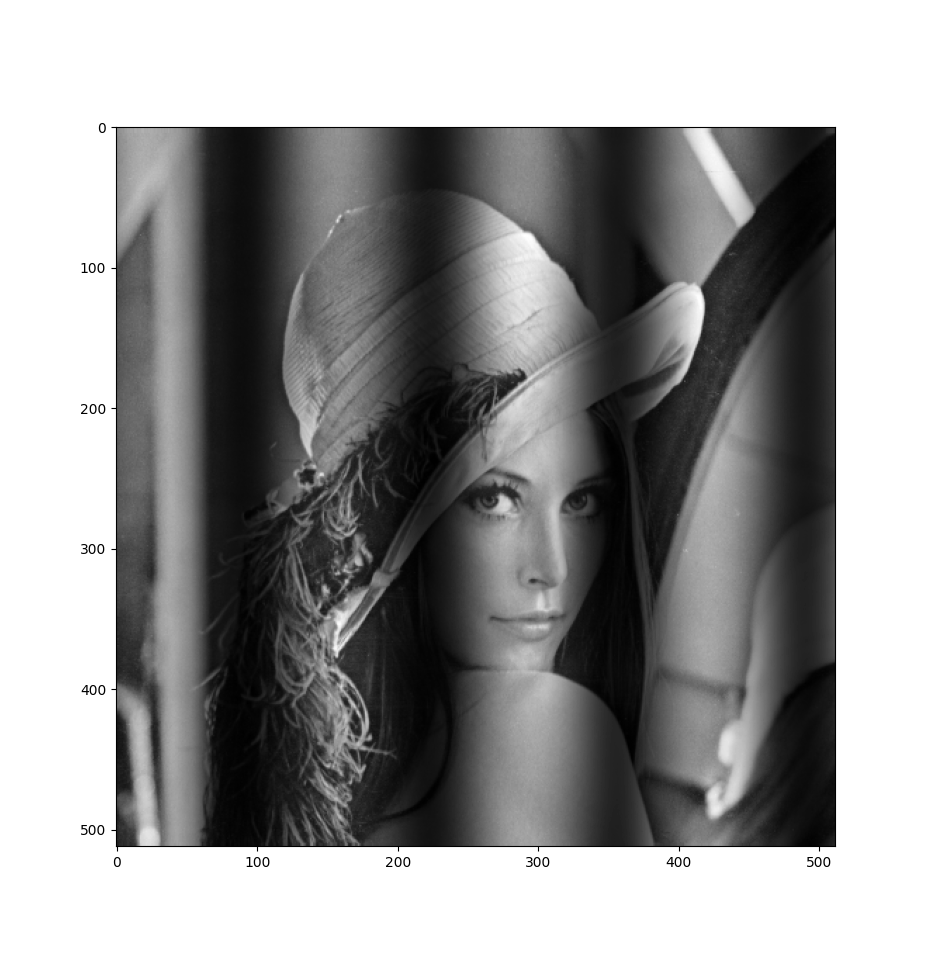
\includegraphics[width=120px]{images/04-applications-image-lena-cos.png} 
        \end{column}    
        \hspace*{-30px}
        \begin{column}{5px}
            $\overset{FT}{\longrightarrow}$
        \end{column}
        \hspace*{-30px}
        \begin{column}{120px}
            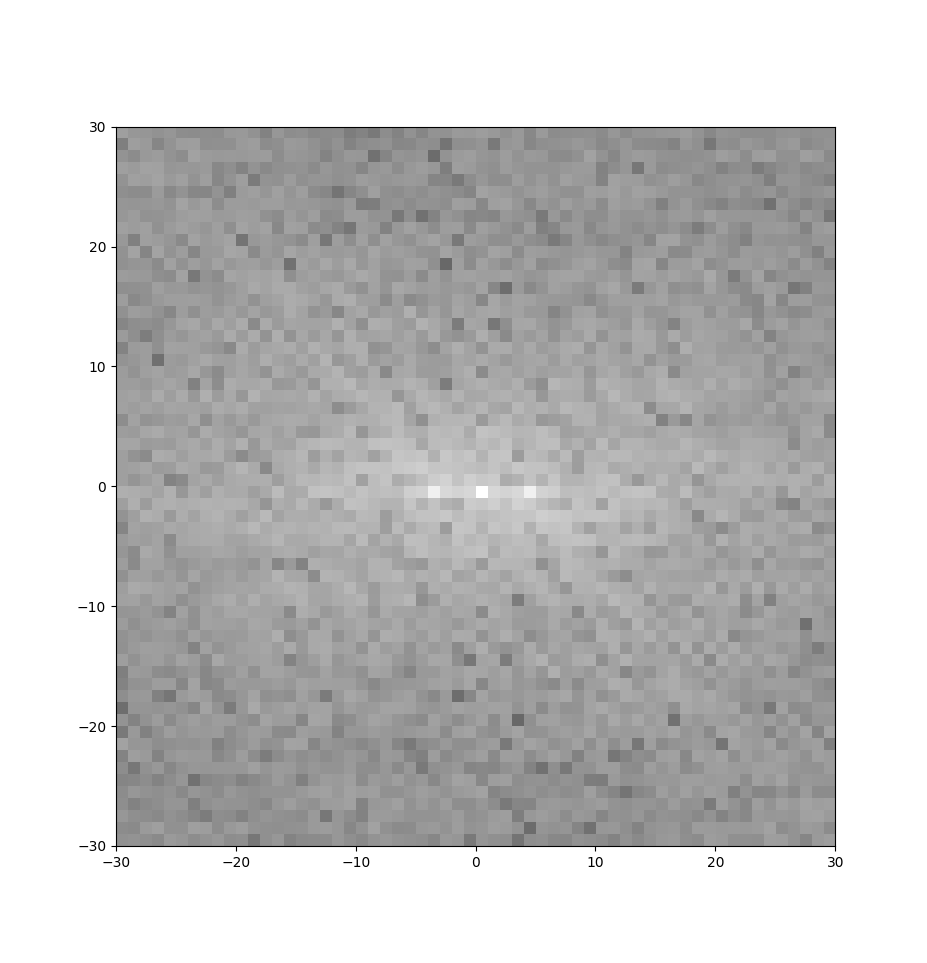
\includegraphics[width=120px]{images/04-applications-image-lena-cos-ft.png}
        \end{column}
    \end{columns}
\end{frame}

\begin{frame}
    \frametitle{Bildverarbeitung}
    \framesubtitle{Rauschfilterung}

    \begin{itemize}
        \item Rauschfrequenz aus Spektrum entfernen
    \end{itemize}

    \begin{columns}
        \begin{column}{120px}
            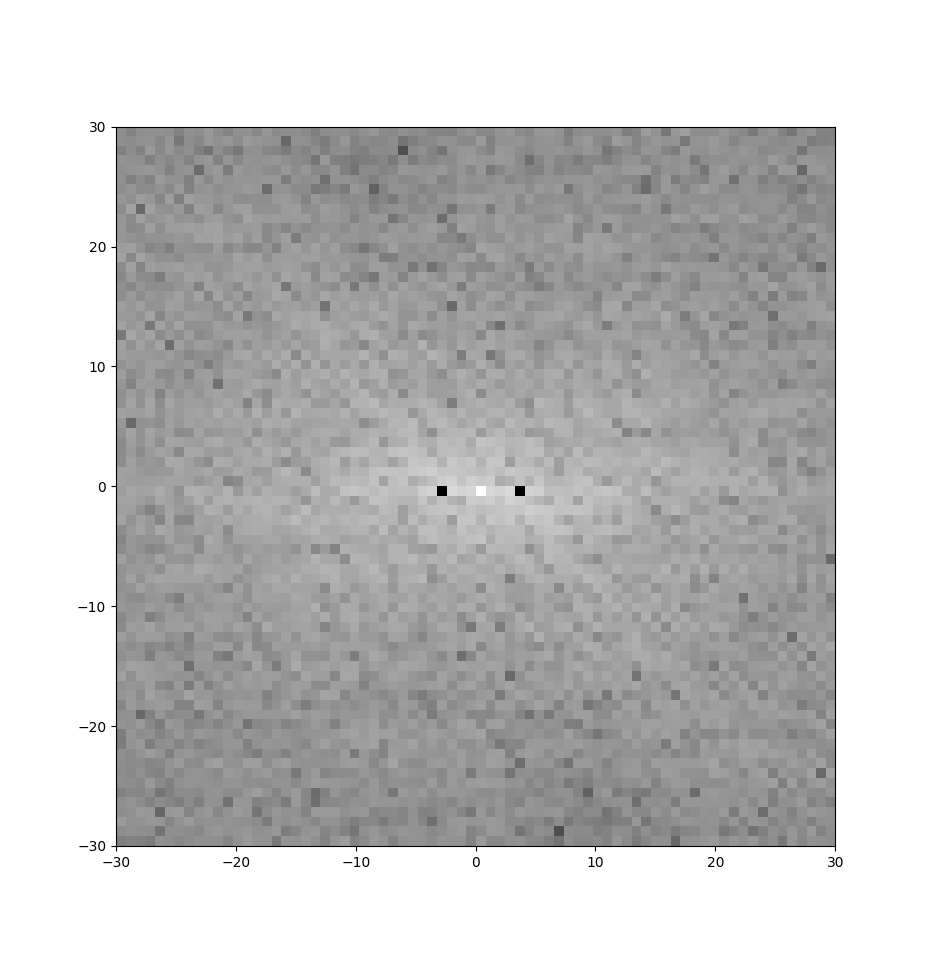
\includegraphics[width=120px]{images/04-applications-image-lena-cos-ft-fixed.png} 
        \end{column}    
        \hspace*{-30px}
        \begin{column}{5px}
            $\overset{FT}{\longrightarrow}$
        \end{column}
        \hspace*{-30px}
        \begin{column}{120px}
            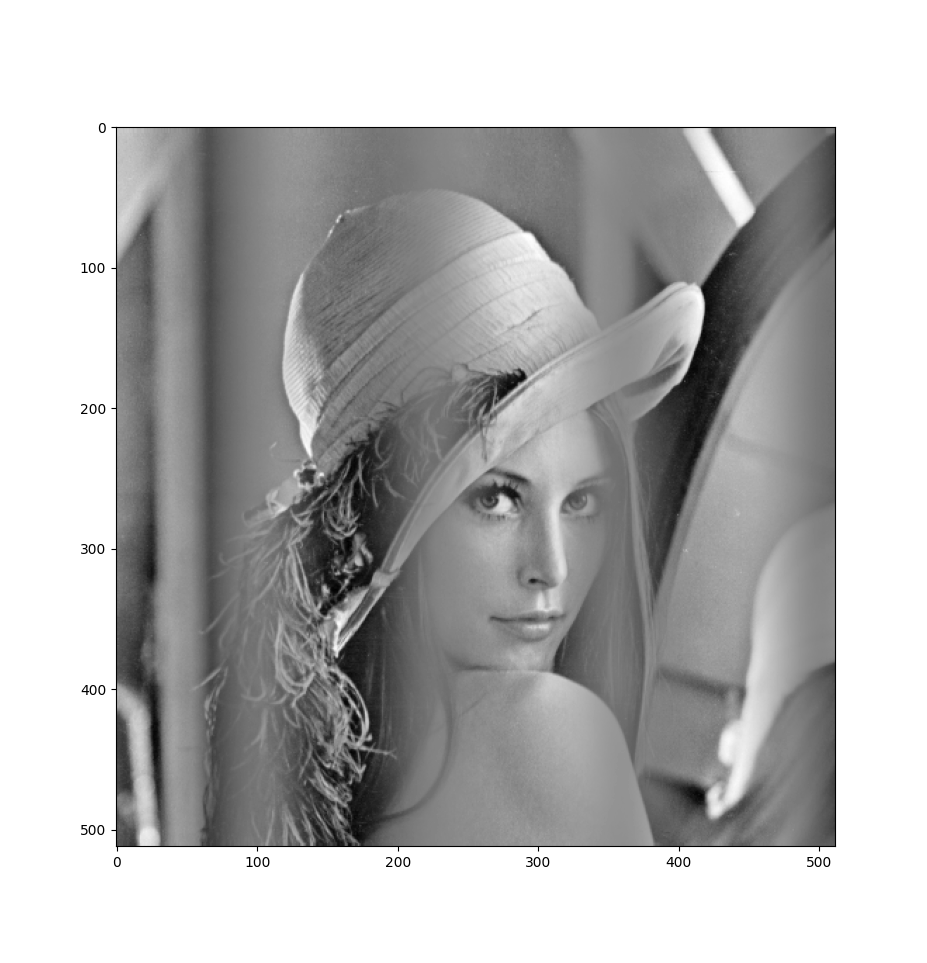
\includegraphics[width=120px]{images/04-applications-image-lena-cos-fixed.png}
        \end{column}
    \end{columns}
\end{frame}
